\documentclass[ngerman]{report}

\usepackage[
        bibencoding=utf8, 
        style=alphabetic
    ]{biblatex}

\usepackage{graphicx}
\usepackage{amsmath}
\usepackage{caption}

\bibliography{bibliography}

\title{Evaluierung von Transferlernen mit Deep Direct Cascade Networks}

\author{Simon Tarras}

\begin{document}
    \maketitle
    \tableofcontents
    % Vollständige Struktur anlegen
    % Einleitung
    % Auch etwas über den Code schreiben (Methoden der Vorstellung (Bsp. Klassendiagram))
    \chapter{Einleitung}  % 1.Einleitung
    \section{Einführung}
    % Wo sind wir gerade?
% Cascade Verfahren entdeckt + festgestellt, dass die recht gut sein könnten.
% Deep Cascade entdeckt + Constructive Networks
% TF angefangen

Selbst diejenigen, die nichts mit Informatik zu tun haben, kennen heute KI. 
Dahinter stecken neuronale Netze. Diese werden meistens in einem Zug komplett gebaut und trainiert. 
Das dauert lange, sodass das Kaskadierungsverfahren der Cascade Correlation \cite{cascor} entwickelt wurde. 
Dabei wurde bemerkt, dass es in Ordnung funktioniert und das schon bei kleineren Netzen. Deshalb wurden darauf aufbauend 
weitere Netzwerke und Kaskadierungsverfahren entwickelt \cite{cascade_network_architectures}, \cite{Constructive_Cascade}, 
\cite{deep_cascade_learning}. Es wurden bei den Kaskadennetzwerken ebenso festgestellt, dass es mit diesem Aufbau der Netze 
einfach ist, einen Wechsel zwischen unterschiedlichen Daten und Aufgaben durchzuführen \cite{phd_deep_cascade}, \cite{transfer_learning}, 
\cite{survey_transfer}. In dem Bereich des Wechsels zwischen unterschiedlichen Daten ist diese Arbeit anzusiedeln, denn sie überprüft, wie 
gut die einzelnen Netzwerkvarianten sind und geht auf die Probleme von TF und Cascade ein. 

% Was fehlt denn noch in der Einführung? 

% Hier kann doch nur eine hinführung zum Thema sein. 

% oder eine Zusammenfassung dessen, was ich tat und was hier vorkommt. 

% Hinführung + Grob, was man tat.

    \section{Motivation}
    Es gibt Aufgaben, die gerne von einer KI übernommen werden sollen, für die es nur sehr kleine Datensätze gibt. Diese sind so klein, dass das 
neuronale Netzwerk hinter der KI nicht genügend Daten für das Training hat, um ein ausreichend gutes und belastbares Ergebnis zu liefern. 
Es ist dabei auch egal, wie lange trainiert wird, es bleibt schlecht. 

Gleichzeitig gibt es den Punkt, dass es meistens ziemlich lange dauert, ein Netzwerk komplett zu trainieren. Beides soll verbessert werden. 

Die Situation mit den zu wenig Daten wird darüber versucht zu verbessern, indem etwas anderes, aber ähnliches, gelernt wird. Dies folgt dem 
Prinzip, wie die Menschen andere ähnliche Dinge lernen können, wenn sie das eine bereits können. Ebenso verlaufen Eselsbrücken für Menschen 
einem ähnlichem Prinzip. Diese Art des Lernens, die über bereits Bekanntes etwas neues lernt, soll nun auch für KI angewandt werden. 

Die Trainingsdauer wird so reduziert, dass das, was tatsächlich im selbem Augenblick trainiert wird, nur sehr wenig ist. Dies soll über die 
Kaskadierungsverfahren Deep Cascade und Direct Cascade gehen. 

    \section{Related Work}
    Diese Arbeit baut auf den CasCor-Algorithmus \cite{cascor}, der wegen der langen Trainingsdauer entwickelt wurde, auf und nutzt diesen, 
um Direct Cascade \cite{cascade_network_architectures} 
durchzuführen, wie es in der Thesis von Marquez \cite{phd_deep_cascade} verwendet wurde. Zudem wird Deep Cascade verwendet als 
Vergleichsbasis \cite{deep_cascade_learning}. Dabei sind Deep Cascade Netzwerke solche, die iterativ aufgebaut werden \cite{Constructive_Cascade}. 
Es wird nur Domain-Wechsel angewandt, während es noch den Taskwechsel \cite{transfer_learning} gibt. Zudem gibt es bei Transfer Learning drei 
Probleme \cite{survey_transfer}, die hier auch bearbeitet werden. \\

Im Folgenden ist die Literaturrecherche: 

% Alle wissenschaftlichen Arbeiten, die hier dazu gehören und verwandt sind aufzählen. 

% Also die Direct Cascade Arbeiten von Ritter und Littmann zum Beispiel. 

% Ebenso Cascor von Fahlmann und Lebiere.

% Deep Cascade Learning von Enrico S. Marquez. 

% Wie sieht das mit dem Bachelorvortrag aus? Wieviel später kommt der?
% Passt das hier von der Länge und dem Inhalt? 


    \chapter{Methodik}  % 2.Methodik
    \section{Transferlernen}
    Transferlernen (Transfer Learning, TL) basiert auf dem Prinzip der Wissensübertragung zwischen unterschiedlichen, jedoch verwandten 
Lernsituationen – vergleichbar mit dem Konzept einer "Eselsbrücke". Es existieren verschiedene Formen des Transferlernens, wobei 
insbesondere zwischen Task Transfer (Aufgabenwechsel) und Domain Transfer (Domänenwechsel) unterschieden wird. Wird keine dieser Varianten 
angewendet, handelt es sich nicht um Transferlernen im engeren Sinne.

In dieser Arbeit wird ausschließlich der Domain Transfer betrachtet, da ausschließlich dieser zum Einsatz kommt. Dabei wird ein Modell, das auf 
einem bestimmten Datensatz (Source-Domain) trainiert wurde, zur Verbesserung der Leistung auf einem anderen, inhaltlich verwandten Datensatz 
(Target-Domain) genutzt – unter Beibehaltung der gleichen Modellarchitektur. Dieser Ansatz wird als Transductive Transfer Learning bezeichnet 
\cite{survey_transfer}. Ziel ist es, das in der Source-Domain erworbene Wissen auf die Target-Domain zu übertragen.

Ein zentrales Problem des Transferlernens besteht darin, geeignete Antworten auf die drei grundlegenden Fragen zu finden: What to transfer, How 
to transfer und When to transfer \cite{survey_transfer}. Diese Aspekte sind bislang nicht abschließend geklärt und stellen weiterhin offene 
Forschungsfragen dar.

Da sowohl Klassifikations- als auch Regressionsmodelle evaluiert werden, kommen jeweils zwei Datensätze als Source und Target zum Einsatz:

\textbf{Klassifikation:}
\begin{enumerate}
    \item Source-Datensatz: Modified National Institute of Standards and Technology (MNIST) \cite{handwritten_digit}
    \item Target-Datensatz: Street View House Numbers (SVHN) \cite{house_numbers}
\end{enumerate}

Beide Datensätze müssen zur strukturellen Kompatibilität für das Transferlernen angepasst werden. MNIST-Bilder (ursprünglich 28x28 Pixel, 
einfarbig) werden auf 32x32 Pixel skaliert. Der SVHN-Datensatz, ursprünglich in Farbe (RGB), wird in Graustufen konvertiert. Dies gewährleistet, 
dass beide Eingabedatensätze die gleiche Dimensionalität aufweisen und somit als Input für dasselbe neuronale Netz genutzt werden können.

\textbf{Regression:}
\begin{enumerate}
    \item Source-Datensatz: Boston Housing Prices (BOST) \cite{Boston_housing}
    \item Target-Datensatz: California Housing Prices (CALI) \cite{California_housing}
\end{enumerate}

Beide Regressionsdatensätze müssen inhaltlich reduziert werden, da nur solche Merkmale berücksichtigt werden sollen, die eine semantisch und 
strukturell sinnvolle Entsprechung in beiden Domänen aufweisen. Im BOST-Datensatz verbleiben nur die drei Merkmale:

\begin{enumerate}
    \item RM: durchschnittliche Anzahl von Zimmern pro Wohnung
    \item AGE: Anteil der vor 1940 erbauten Häuser
    \item LSTAT: Anteil der Bevölkerung mit niedrigem sozioökonomischem Status
\end{enumerate}

Hinweis: Die ursprünglich im BOST-Datensatz enthaltene Variable mit ethnisch diskriminierendem Inhalt wird vollständig entfernt.

Im CALI-Datensatz verbleiben:
\begin{enumerate}
    \item MedInc: mittleres Einkommen pro Häuserblock
    \item HouseAge: durchschnittliches Alter der Gebäude
    \item RoomsPerHousehold: abgeleitet durch Division von AveRooms (durchschnittliche Zimmeranzahl im Block) durch Households (Anzahl der Haushalte)
\end{enumerate}

Diese Ableitung stellt die strukturelle Entsprechung zur RM-Variable im BOST-Datensatz dar.

Eine inhaltliche Verbindung besteht voraussichtlich zwischen LSTAT (BOST) und MedInc (CALI), da sozioökonomischer Status und Einkommen 
erfahrungsgemäß korrelieren. Da LSTAT jedoch antiproportional zur Einkommenshöhe ist, wird diese Variable invertiert, um eine proportionale 
Beziehung zur MedInc-Variable herzustellen – eine Voraussetzung für effektives Transferlernen.

Die Harmonisierung der Altersvariablen gestaltet sich komplexer: AGE im BOST-Datensatz beschreibt den Anteil der vor 1940 erbauten Häuser, 
während HouseAge im CALI-Datensatz das durchschnittliche Alter der Gebäude angibt. Um AGE in eine vergleichbare Form zu bringen, wird auf 
Basis einer angenommenen maximalen Anzahl von 100 Häusern pro Block und einem maximalen Alter von 85 Jahren (bezogen auf das Jahr 2025) eine 
Umrechnung vorgenommen. Die entsprechende Formel lautet:
\begin{equation}
    \frac{AGE * 85}{Maximalanzahl}
\end{equation}

Durch die beschriebenen Anpassungen weisen alle verwendeten Source- und Target-Datensätze strukturelle Kompatibilität zueinander auf. Damit ist 
die Frage "Was wird transferiert?" im Sinne des Transferlernens hinreichend beantwortet.

Die nächste zu klärende Dimension ist das "How to Transfer". Der Transfer erfolgt in allen Fällen ohne Modifikation der Gewichtungen zuvor 
trainierter Netzwerkschichten. Das neuronale Netzwerk wird zunächst vollständig auf dem Source-Datensatz trainiert. Anschließend erfolgt der 
Übergang zum Target-Datensatz, ohne dass das Modell selbst oder dessen Gewichtungen verändert werden.

Dabei unterscheiden sich die beiden eingesetzten Kaskadierungsansätze hinsichtlich der Art des Transfers:
\begin{enumerate}
    \item Beim Deep Cascade-Verfahren bleibt die Netzinputgröße unverändert, und lediglich die Eingabedatenquelle (Source → Target) wird gewechselt. 
    Der Transfer vollzieht sich somit ausschließlich über die Änderung des Input-Datensatzes bei gleichbleibender Architektur und 
    Parameterbelegung. Dabei ist zu bedenken, dass dieses Netz immer größer wird.
    \item Beim Direct Cascade-Verfahren erfolgt der Transfer implizit über die kontinuierliche Erweiterung des Eingaberaums. Der sogenannte 
    Augmented Input wird bei jedem Schritt vergrößert, sodass die auf dem Source-Datensatz erlernten Repräsentationen in den nachfolgenden 
    Stufen weiterhin einfließen.
\end{enumerate}
    
    
Die Frage "Wann ist Transfer Learning sinnvoll?" (When to Transfer) kann bislang nicht eindeutig beantwortet werden. Aus diesem Grund wird in 
den Experimenten mit unterschiedlichen Zeitpunkten für den Transfer gearbeitet – sowohl mit einem frühen als auch mit einem späteren Übergang 
zum Target-Datensatz.

    \section{Kaskadierung}
    Hier wird erklärt, was ein Kaskadennetzwerk ist und welche Besonderheiten es dabei gibt. 
Ein Kaskadennetzwerk ist ein Netzwerk, welches in Kaskaden, also Schrittweise, aufgebaut wird. Während bei einem klassischen Netz 
vorher festgelegt wird, wieviele und welche Layer dieses haben wird, ist es bei einem Kaskadennetzwerk nicht so. Ein solches Netzwerk 
wird erst während dem Training aufgebaut und immer erweitert. Deshalb werden, im Gegensatz zu den klassischen Netzen, nur der aktuelle neue 
Teil trainiert, während der Rest nicht mehr verändert wird. Die vorher gelernten Layer werden nach dem Training gefreezt. Dadurch 
werden die Gewichte mehr der gefreezten Layer nicht mehr verändert. Die Kaskadennetzwerke lernen dadurch das, was zwischen den Layern 
gelernt wird, nicht und sind deshalb etwas schlechter als die klassischen Netzwerke bei gleich vielen Daten. Aber, weil immer nur das 
aktuelle gelernt wird, sind Kaskadennetzwerke im Training sehr viel schneller. Dies liegt daran, dass die Gewichte der vorherigen Layer 
kein sich verändertes Bild von den nachfolgenden Gewichten in jeder Epoche haben und sich nicht aktualisieren müssen. 

    \subsection{Deep Cascade}
    Hier wird die Variante des Deep Cascade vorgestellt. 
Die Deep Cascade Netze werden iterativ während dem Training aufgebaut. Es bleibt dabei ein einziges Netz. Es wird zuerst 
definiert, welcher Optimizer und welcher Loss in dem Netz genutzt wird. 

\begin{figure}[htpb]
    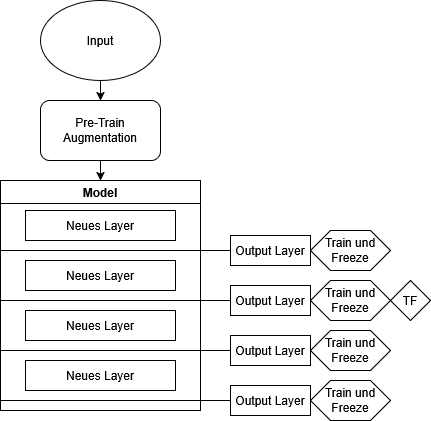
\includegraphics[height=10cm]{../../Graphiken/deepcascade_2.png}
    \caption{\label{fig:deepcascade} Vorstellung Deep Cascade Aufbau}
\end{figure}

Sobald dies beides gemacht wurde, wird im Netz das erste Layer definiert. Dieses wird ergänzt durch ein Output Layer und dann trainiert. 
Wenn das Training beendet wird, wird das Output Layer gelöscht und ein neues Layer hinzugefügt, wie es in Figure 2.1 gezeigt wird. Zudem wird 
das gerade trainierte Layer gefreezt, damit dieses keine weiteren Aktualisierungen mehr bekommt. 
Dann wiederholt sich das Training, das Löschen, das Freezing und weitere Hinzufügen von Layern. 
An einer beliebigen Stelle kann TF gemacht werden, indem, statt in der Trainingsphase den Sourcedatensatz zu nutzen, der Targetdatensatz 
genutzt wird. 

% Sollte ich nicht vorher Kaskadierung erklären? Oder geht das hier? Hier könnte ich auch Graphen bauen. Ist glaube ich sogar besser, wenn 
% ich es tue...

    \subsection{Direct Cascade}
    In diesem Abschnitt wird die Kaskadierungsvariante des Direct Cascade Netz-werks vorgestellt. Das Netzwerk ist hierbei vollständig vorab 
definiert und besteht aus einem einzelnen Hidden Layer sowie einem Output-Layer. Die Gesamtstruktur setzt sich aus mehreren identischen 
Subnetzwerken zusammen, zwischen denen während des Trainings ein Wissenstransfer stattfindet.

\begin{figure}[htpb]
    \centering
    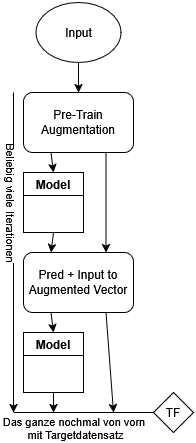
\includegraphics[height=10cm]{../../Graphiken/direct_cascade.png}
    \caption{\label{fig:directcascade} 
    \small{Hier wird das Direct Cascade Verfahren dargestellt. Dieses Verfahren verwendet mehrere einzelne Netzwerke 
    (hier als Modelle bezeichnet), die jeweils nur wenige Hidden Layer aufweisen, in der Regel lediglich einen. Nach der 
    Initialisierung und dem Training wird jedes Modell einmal ohne weiteres Training angewendet, dessen Ausgangssignal mit dem ursprünglichen 
    Eingabesignal kombiniert wird. Diese Kombination bildet den neuen Eingabedatensatz für das nachfolgende Modell. Durch diese sukzessive 
    Verknüpfung der Ausgaben mit den Eingaben kann das Verfahren eine Wissensweitergabe und -integration zwischen den einzelnen Modellen 
    realisieren. Darüber kann an beliebiger Stelle TF verwendet werden.}}
\end{figure}

Der Ablauf beginnt, wie in Abbildung \ref{fig:directcascade} dargestellt, mit dem vorberei-teten Source-Datensatz, der als 
Eingabe in die erste Instanz des Netzwerks gegeben wird. Diese Netzwerkinstanz wird anschließend trainiert. Nach Abschluss des Trainings 
erfolgt eine einmalige Anwendung des fixierten Netzwerks, deren Ergebnis die Vorhersage (Prediction) darstellt. Diese Prediction wird mit 
dem ursprünglichen Eingabesignal desselben Netzwerks kombiniert, wodurch ein sogenannter Augmented Vector entsteht. Die genaue Bildung dieses 
Augmented Vectors variiert dabei leicht je nach spezifischer Implementierung des jeweiligen Direct Cascade Netzwerks und wird an späterer 
Stelle detaillierter erläutert.

Der Augmented Vector dient als Input für die nächste Instanz des Netzwerks. Dieser Zyklus aus Netzwerkinstanz, Training, Prediction und 
Augmented Vector Berechnung wird beliebig oft wiederholt. Durch die Einbindung der Prediction in den Augmented Vector kann das Netzwerk 
Wissen aus den zuvor trainierten Instanzen übernehmen und integrieren.

TF kann jederzeit innerhalb eines Trainingsschritts durchgeführt werden, indem anstelle des Source-Datensatzes 
ein Target-Datensatz als Input verwendet wird. Dabei können beliebig viele Netzwerkinstanzen vor und nach 
TF genutzt werden. Der einzige Unterschied besteht darin, dass der Augmented Vector mit jedem weiteren Netzwerk etwas 
größer wird, da er sowohl das Wissen aller bisher trainierten Netzwerke als auch die ursprünglichen Eingabedaten enthält.

Für die Implementierung bedeutet dies, dass von Beginn an sowohl der Source- als auch der Target-Datensatz in das feste Netzwerk eingespeist 
werden müssen. Dies ist notwendig, um die Prediction auf dem Target-Datensatz – die während der Trainingsphase mit dem Source-Datensatz generiert 
wurde – im Augmented Vector zu integrieren. Somit wird sichergestellt, dass das während des Trainings auf dem Source-Datensatz gelernten 
Wissens auch bei der Anpassung an den Target-Datensatz berücksichtigt werden.

    \section{Setup}
    Alle Test wurden auf einem Erazer Gaming Notebook P15601 unter Windows 10 durchgeführt.
Die Neuronalen Netze laufen dabei ausschließlich auf 
der CPU und wurden nur trainiert, wenn der Rechner am Stromnetz angeschlossen war. 
Dieser Rechner hat einen intel Core i5 der neunten Generation mit 4 Kernen auf 8 
logischen Prozessoren. Die Betriebsgeschwindigkeit liegt bei 2,4-5,1 GHz und die 
RAM-Größe liegt bei 15,8 GB bei einer Geschwindigkeit von 2667 MHz. 

Es wurde mit PyCharm und der library Keras programmiert. Die Texte sind mit BibTex 
erstellt worden und die Plots mit der MatPlotLib library.

Die genutzten Datensätze sind Modified National Institute of Standards and Technology Dataset (MNIST), 
Streetview House Numbers (SVHN), Boston Housing Prices (Boston) und California Hausing Prices (California).

Dabei sind MNIST und Boston die Sourcedaten und SVHN und California die Targetdaten. Jeder Targetdatensatz 
wird händisch verkleinert, da es darum geht, nicht genügend Daten für sie allein zu haben und eine andere 
Methode genutzt werden muss.

    % \section{Durchführungen}
    % Es wurden sowohl für Klassifikation als auch für Regression drei verschiedene Ansätze der Kaskadierung genutzt. 
Ebenso wurde Direct TF mit Domainwechsel durchgeführt. 

Die drei Ansätze sind Deep Cascade, Direct Cascade und eine Kaskadierung von einem Netz im Netz mit mehreren Inputs.

Bei Deep Cascade wird ein Netz Layer für Layer aufgebaut und jedes Layer einzelnd trainiert und gefreezt. 
Bei Direct Cascade werden ganze Netze trainiert und dessen Prediction als zusätzlichen Input für das nächste Netz zu nutzen.
Bei der dritten Variante wird ein Netz trainiert, dann auf einem Teilnetz davon die Prediction gemacht, um mit dieser das 
ganze Netz außer das vorher erwähnte Teilnetz zu trainieren. 
Nur Deep Cascade wird genauer betrachtet, denn die beiden anderen Ansätze sind nur zum Vergleichen da.

Es wurde bei jedem gleichbleibende Epochenanzahlen, zufällige und von einer Metrik abhängige durchgeführt. 

Bei allen Neuronalen Netzen wurden die dafür benötigten Daten in ein Trainings-, Validation- und Testdatensatz aufgeteilt. 
Ebenfalls wurde MNIST auf 32x32 erweitert, sowie SVHN in graue Bilder mit einem Channel verändert. 
Es wurde erweitert, da keine Daten unnötig verloren werden sollten. Die Reduzierung von SVHN liegt daran, dass MNIST nur 
Schwarz-Weiß-Bilder sind und es nicht möglich ist, dies in bunte Bilder zu verändern.
Die Veränderungen der Datensätze kommt daher, dass sie technisch gleich aussehen müssen, da sie sonst nicht als Input 
desselben Netzes genutzt werden können.

Für die Regressionsnetze müssen alle Spalten weggenommen werden, die kein Gegenüber im anderen Datensatz besitzen. 
Somit fielen die Spalten: Verbrechensrate, Anteil der Wohngebiete über 25000 Fuß, Nicht-Einzelhandelanteil der Gewerbeflächen, 
Flussgrundstück, Stickoxidkonzentration, Entfernung zu Arbeitsvermittlungszentren, Erreichbarkeit von Autobahnen, 
Vollwertsteuersatz, Schüler-Lehrer-Verhältnis und die Anzahl von Schwarzen im Bosten weg, während im California die 
folgenden Spalten wegfielen: Längengrad, Breitengrad, Schlafzimmer und Bevölkerung. Aus der Gesamtanzahl der Räume und der Haushalte 
wird die durchschnittliche Anzahl an Räumen pro Wohnung errechnet.
Diese Spalten haben alle keinen Gegenüber im anderen Datensatz und eine Spalte ist aus ethnischen Gründen nicht nutzbar, was daran liegt, 
dass der Datensatz aus den Siebzigern stammt.
Übrig blieben von Boston nur noch die durchschnittliche Anzahl der Räume pro Wohnung, die Menge der Häuser, die vor 1940 
erbaut worden sind und der prozentuale Anteil der Bevölkerung mit niedrigem Status.
Bei California blieben das Errechnete und das Hausalter, sowie das durchschnittliche Einkommen. 
Die Anzahl der Räume pro Wohnung passen offensichtlich zueinander, während der prozentuale Anteil der Bevölkerung mit niedrigem Status 
antiproportional zu dem durchschnittlichen Einkommen ist. Dies wird vorher zu einer Proportionalität umgewandelt.
Als etwas komplizierter erweist sich das Alter. Mit Prozentrechnung kann man aber das ungefäre Alter der Häuser aus dem 
Boston Datensatz abschätzen. Da immer eine Häuseranzahl von einhundert betrachtet wird, ist dies die Gesamtmenge und folgende Formel 
löst das Problem: 
\begin{equation}
    \frac{Hausanzahl * Hausalter}{Gesamtmenge}
\end{equation}
Die Hausanzahl ist hier die Menge der Häuser, die vor 1940 erbaut worden sind. Das Hausalter bezieht sich auf das Alter der eben 
erwähnten Häuser und ist auf Heute angedacht; sind also 85 Jahre.

Die Hypothese war, dass man mit TF bei zu wenig Daten eine verhältnismäßig gute Performanz der Netze erwarten kann, sowie, 
dass durch einen Kaskadierungsansatz das Training der Netze sehr kurz ist.

Generell wird zuerst eine Weile auf dem Sourcedatensatz trainiert und dann auf den Targetdatensatz gewechselt ohne die 
bisherigen Netze zu verändern. Bis auf den Direct Cascade Ansatz werden auch die Inputs während des ganzen Prozesses nicht 
verändert.
Bei Direct Cascade werden die Inputs immer größer, denn die Prediction des vorherigen Netzes wird zum Input hinzugefügt.

    \section{Metrik}
    Es wurden drei Evaluationsmetriken definiert: die Accuracy-Metrik (ACCM), die Loss-Metrik (LM) sowie die Mean Absolute Error-Metrik (MAEM). 
Diese Metriken dienen als Kriterien für das Early Stopping und bestimmen die Anzahl der Trainings-Epochen.

Das Early Stopping anhand der ACCM erfolgt, sobald die Validierungsgenauigkeit um mindestens 10\% unter der 
Trainingsgenauigkeit liegt, was auf Overfitting im Netzwerk hinweist.

Bei der LM und MAEM wird das Training beendet, wenn der Validierungswert in der aktuellen Epoche schlechter ausfällt als in der 
vorherigen. Dieses Verhalten verursacht, dass das Netzwerk in einem lokalen Minimum konvergiert, aus dem es nicht mehr herausfindet.

Für die Anzahl der Netzwerke im Direct Cascade Verfahren wird keine dieser Metriken zur Steuerung des Trainings eingesetzt. 
Ihre Anwendung besteht darin, den Trainingsprozess vorzeitig zu beenden, noch bevor die vorgesehene maximale Anzahl an Epochen erreicht wird. 

    \section{Liste der Tests}
    
Liste aller hier vorkommenden Netzen mit ihren Kürzeln:

\begin{enumerate}
    \item ConvMaxPool (CMP)
    \item 1DConv (1DC)
    \item 2DConv (2DC)
    \item ClassOneDense (COD)
    \item RegressionTwo (Regr2)
    \item OneLayer (1Lay)
\end{enumerate}

Davon sind ConvMaxPool und RegressionTwo Deep Cascade Netzwerke, während alle anderen Direct Cascade Netzwerke sind. 
Ebenso sind nur RegressionTwo und OneLayer Regressionsnetze, während der Rest Klassifikationsnetze sind. 

Alle Netze werden mit dem Adam-Optimizer mit der Lernrate 1e-3 gelernt. Klassifikationsnetze haben als Loss den 
CategoricalCrossEntropy und Softmax als Aktivierungsfunktion, während die Regressionsnetze MeanSquaredError und Linear als 
Aktivierungsfunktion vorweisen. 

Mit allen Direct Cascade Netzwerken wurden zusätzlich Early Stopping Metriken durchgeführt mit MAEM, LM und ACCM. 

Für alle Klassifikationsnetze gilt, dass sie mit fünf verschiedenen Größen des Targetdatensatzes trainiert wurden. Die Ausnahme ist das 
2DC-Netzwerk, welches nur mit sehr wenigen Source- und Targetdaten trainiert werden kann, da es technisch auf derselben Hardware mit mehr 
Daten unmöglich ist. 

Bei den Regressionsnetzen wird jeweils einmal mit vielen und wenigen Targetdaten trainiert. 

Es wurde mit allen Netzwerken ein Vergleich sowohl zwischen mit TF und ohne als auch zwischen ohne TF und Kompletten angefertigt. 
Komplett heißt hier, dass es ein Netzwerk ohne TF und ohne Kaskadierung ist und dieses deshalb in einem komplett trainiert wird. 

Mit allen Netzwerken wurde der Zeitpunkt für das TF frei ausgetestet. 

Alle Direct Cascade Netzwerke haben jeweils nur ein Hidden Layer. In manchen Fällen sind sie noch mit einem Hilfslayer, um den Wechsel 
zwischen Filterlayern und Linearlayern zu bewerkstelligen. 

Für alle Netzwerke wurde derselbe Seed für die Initialisierung der Weights genutzt. 

In Tabelle 2.1 sind die Tests bezüglich Klassifikation und in Tabelle 2.2 die für die Regression. 
In beiden Tabellen sind die Tests, die sich mit der Zeitdauer befassen mit der Endung Time. Dabei gilt, dass CasTF Kaskadierung mit TF, Cas allein 
Kaskadierung ohne TF und Comp bedeutet, dass es weder TF noch Kaskadierung gab. ACCM, LM und MAEM sind die Tests bezüglich der Early-Stopping 
Metriken. 
Vor dem ersten Schrägstrich steht, wann TF gemacht wurde, welches mit TF im Eintrag gekennzeichnet ist. Wenn kein TF gemacht wurde, ist dieser 
erste Bereich nicht existent. Dahinter steht die Datenmenge 
des Targetdatensatzes und danach die Menge an Epochen pro Trainingsiteration. Wenn es noch etwas viertes gibt, dann zeigt dieses an, wieviele 
Epochen in Zehnern es insgesamt gab. 

\begin{table}[!ht]
    \centering
    \begin{tabular}{l|l|l|l}
        \textbf{CMP} & \textbf{COD} & \textbf{1DC} & \textbf{2DC} \\
        \hline
        TF0/732/10 & CasTFTime & CasTFTime & CasTFTime \\
        TF1/732/10 & CasTime & CasTime & CasTime \\
        TF2/732/10 & CompTime & CompTime & CompTime \\
        TF3/732/10 & TF2/732/10 & TF2/732/10 & TF2/732/10 \\
        TF4/732/10 & TF2/7k/10 & TF2/7k/10 & \\
        TF5/732/10 & TF2/21k/10 & TF2/21k/10 & \\
        732/10 & TF2/36k/10 & TF2/36k/10 & \\
        CasTFTime & TF2/51k/10 & TF2/51k/10 & \\
        CasTime & TF10/732/10/30 & TF10/732/10/30 & \\
        CompTime & 732/10/30 & 732/10/30 & \\
        TF2/7k/10 & Comp/732//30 & Comp/732//30 & \\
        TF2/21k/10 & ACCM/732/10 & ACCM/732/10 & \\
        TF2/36k/10 & LM/732/10 & LM/732/10 & \\
        TF2/51k/10 & & & \\
        & & & \\
    \end{tabular}
    \caption{\label{tab:classtests} Liste aller Klassifikationstests}
\end{table}

\begin{table}[!ht]
    \centering
    \begin{tabular}{l|l}
        \textbf{Regr2} & \textbf{1Lay} \\
        \hline
        TF0/240/25 & CasTFTime \\
        TF1/240/25 & CasTime \\
        TF4/240/25 & CompTime \\
        CasTFTime & TF11/8k/10/8 \\
        CasTime & 8k/10/8 \\
        CompTime & Comp/8k/10/8 \\
        TF3/8k/10/8 & TF11/240/10/20 \\
        8k/10/8 & 240/10 \\
        Comp/8k/8 & Comp/240/8 \\
        TF3/240/8 & MAEM/240/10 \\
        240/8 & LM/240/10 \\
        Comp/240/8 & TF4/206/10/8/ts \\
        TF4/206/10/8/ts & 206/10/8/ts \\
        206/10/8/ts & Comp/206/10/8/ts \\
        Comp/206/10/8/ts &
    \end{tabular}
    \caption{\label{tab:regrtests} Liste aller Regressionstests}
\end{table}

Eine Referenz zu einer dieser Listen ist CMP:TF0/732/10. Diese bedeutet, dass es um den Test mit der Kennung TF0/732/10 des CMP-Netzwerkes geht. 
Bei diesem gibt es die Besonderheit, dass TF nach dem ersten Layer gemacht wird, dieses Layer jedoch im 
Gegensatz zum restlichen Netzwerk nur mit einer Epoche trainiert wird.
Selbiges gilt für Regr2:TF0/240/25.

Die Tests mit der Endung ts sind diejenigen, die einen explizit großen Testdatensatz haben. 


    \chapter{Allgemeine Resultate}  % 3.Allgemeines
    \section{ConvMaxPool}
    Anhand des ConvMaxPool-Netzwerks werden alle allgemeinen Resultate und Auffälligkeiten beschrieben. 
Dies ist ein Deep Cascade Classification Netzwerk und wird deshalb iterativ aufgebaut. 
Das Netz ist ein Convolution-Network mit Padding, sodass die Dimensionen während der Convolution-Layer sich nicht verringert. 
Es wird die Aktivierungsfunktion relu genutzt. 

\begin{figure}[htpb]
    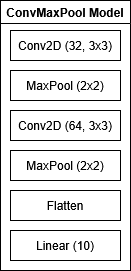
\includegraphics[height=5cm]{../../Graphiken/convmaxpool.png}
    \caption{\label{fig:convmaxpool} Vorstellung des ConvMaxPool Netzwerks}
\end{figure}

\iffalse
\begin{enumerate}
    \item Conv2D (32, (3, 3), same, relu)
    \item MaxPool2D (2, 2)
    \item Conv2D (64, (3, 3), same, relu)
    \item MaxPool2D (2, 2)
    \item Flatten
    \item Dense (10, softmax)
\end{enumerate}
\fi

Alle Layer des ConvMaxPool Netzwerks sind in Figure 3.1 in korrekter Reihenfolge zu sehen. Dabei ist die erste Zahl eines Convolution Layer 
die Anzahl der genutzten Filter, während das folgende Tuple die Kerngröße beschreibt. Ebenfalls die Kerngröße steht bei den MaxPool Layern dort. 
Das Flatten- und das Linear-Layer sind der Output-Block. Das Linear-Layer benötigt zehn Nodes, da es zehn Klassen gibt. Jedes Hidden Layer wird 
mit zehn Epochen trainiert. Es gibt keine Early-Stopping Metrik und es wird derselbe Seed für alle Tests genutzt. 

    \subsection{Einbruch bei TF}
    \subsection{Wenig Epochen für Stabilisierung}
    \subsection{Overfitting auf Sourcedatensatz}
    \section{Zeitnahme}

    \chapter{Klassifikation}  % 4.Klassifikation
    \section{Größe des Targetdatensatzes}
    \section{Bilddimensionalität}
    \section{Augmentierung}
    \section{Mit und Ohne}
    \subsection{TF}
    \subsection{Kaskadierung}

    % \section{Filternetze}
    % Die Klassifikation über Filternetze im Direct Cascade Ansatz. 
Es wird zudem zwischen eindimensionalen und zweidimensionalen Bilddaten unterschieden, um zu zeigen, dass die Dimensionalität für die 
Accuracy irrelevant ist und es im zweidimensionalen nur länger dauert. 

Der zweidimensionale Fall hat folgende Updateregel: 
Die Prediction wird ausgelesen und dessen Wert wird in ein Array mit demselben Shape hineingeschrieben und dies wird dann mit den Trainingsdaten 
auf der Channelachse konkateniert. Dies ergibt den Augmented Vector, der als Input für das nächste Netz genutzt wird.

Die Besonderheit des zweidimensionalen Netzes ist es, dass es in der Updateregel sehr viel Arbeitsspeicher benötigt wird. Deshalb wird nicht nur 
der Targetdatensatz auf 1\% verkleinert, sondern auch der Sourcedatensatz. 

Es wurde einmal ohne Metrik, einmal mit der Accuracy-Metrik und einmal mit der Loss-Letrik ausgetestet.

\begin{figure}[htpb]
    \includegraphics[height=5cm]{../../Plots/DirClass_LilConv/Dir2DLilConvTrainTen2Ten.png}
    \includegraphics[height=5cm]{../../Plots/DirClass_LilConv/Dir2DLilConvTestTen2Ten.png}
    \includegraphics[height=5cm]{../../Plots/DirClass_LilConv/Ten2TenTrain_ACC.png}
    \includegraphics[height=5cm]{../../Plots/DirClass_LilConv/Ten2TenTest_ACC.png}
    \includegraphics[height=5cm]{../../Plots/DirClass_LilConv/Ten2TenTrain_Loss.png}
    \includegraphics[height=5cm]{../../Plots/DirClass_LilConv/Ten2TenTest_Loss.png}
    \caption{\label{fig:2dconv}}
\end{figure}

Die Figure 2.1 zeigt die Plots der Tests zuerst ohne eine Metrik, dann mit der ACCM und zum Schluss mit der LM. 
Da der Sourcedatensatz verringert wurde, ist die Accuracy im ersten Bereich geringer als es erwartbar ist. 
Das Early Stopping ist hier nicht erkennbar, da die Berechnungszeit des Augmented Vector hier für die Zeit entscheidend ist.

Im eindimensionalen Fall gibt es folgende Updateregel: 
Die Bilddaten werden zuerst in eindimensionale Bilder verändert mit Channels. Dies ist der Input des Netzes. Die Prediction und der Netzinput, 
dessen Channelachse vorübergehend entfernt wird, werden direkt konkateniert und das Ergebnis, um die Channelachse erweitert. 

Hier wird nur der Targetdatensatz verkleinert und einem ohne Metrik, mit der ACCM und der LM ausgetestet. Dies zeigt die Figure 2.2.

\begin{figure}[htpb]
    \includegraphics[height=5cm]{../../Plots/DirClass_OneDConv/Ten2TenTrain.png}
    \includegraphics[height=5cm]{../../Plots/DirClass_OneDConv/Ten2TenTest.png}
    \includegraphics[height=5cm]{../../Plots/DirClass_OneDConv/DataTrain_ACC_Metr.png}
    \includegraphics[height=5cm]{../../Plots/DirClass_OneDConv/DataTest_ACC_Metr.png}
    \includegraphics[height=5cm]{../../Plots/DirClass_OneDConv/Ten2TenTrain_Loss.png}
    \includegraphics[height=5cm]{../../Plots/DirClass_OneDConv/Ten2TenTest_Loss.png}
    \caption{\label{fig:1dconv}}
\end{figure}

Hier werden die Metriken eindeutig gesehen, denn die Trainingszeit ist sehr verschieden. Es wird auch klar, dass der eindimensionale Fall 
schlechter ist als der Zweidimensionale.
Dies liegt daran, dass im eindimensionalen nur die Daten rechts und links von dem betrachteten Pixel in die Berechnung mit eingezogen werden 
können, während im zweidimensionalen zusätzlich auch die Daten oben, unten und die vier Ecken jenes Kreuzes betrachtet werden.
% da der eindimensionale Fall nicht die Verhältnisse der Pixel innerhalb einer Achse auf beiden Achsen betrachten kann. 
Beide Netze haben eine sehr schlechte Accuracy. Dies liegt aber nicht daran, dass auf dem Sourcedatensatz Overfitting passiert ist, denn es 
wird nicht besser, wenn der Wechsel der Datensätze beliebig nach vorne geschoben wird.

    % \section{Linearnetze}
    % Die Klassifikation über Linearnetze mittels eines Direct Cascade Ansatzes. 

Das Netz hat ein Linearlayer mit 512 Nodes und der ReLU-Activation function.

Für den augmented Vector werden alle inputdaten in eindimensionale Bilder verwandelt. Der Input wird mit der Prediction konkateniert und 
direkt an das nächste Netz weitergegeben.

Dieses Netz wurde ohne Metrik, mit der ACCM und LM ausgetestet. 

\begin{figure}[htpb]
    \includegraphics[height=5cm]{../../Plots/MnistLongDense/DataTrain.png}
    \includegraphics[height=5cm]{../../Plots/MnistLongDense/DataTest.png}
    \includegraphics[height=5cm]{../../Plots/MnistLongDense/Ten2Ten_Train_ACC.png}
    \includegraphics[height=5cm]{../../Plots/MnistLongDense/Ten2Ten_Test_ACC.png}
    \includegraphics[height=5cm]{../../Plots/MnistLongDense/Ten2Ten_Train_Loss.png}
    \includegraphics[height=5cm]{../../Plots/MnistLongDense/Ten2Ten_Test_Loss.png}
    \caption{\label{fig:linclass}}
\end{figure}

Die Figure 2.3 zeigt, dass ein Netzwerk mit nur Linearlayers etwas schlechter ist als ein zweidimensionales Filternetz. 
Hier werden die Metriken auch bereits gesehen, aber sie bringen kein erhofftes Ergebnis. 

Die Klassifikation funktioniert mit den Updateregeln und diesen Netzen nicht. Auch TF bringt dabei nichts. Das einzige, 
was halbwegs etwas bringt, ist, wenn mehr Targetdaten benutzt werden. Aber dann wird TF auch nicht mehr gebraucht. 


    \chapter{Regression}  % 5.Regression
    \section{Datenaugmentation}
    \subsection{Wenig Daten}
    \subsection{Viele Daten}
    \section{Early Stopping}
    % Diskussion
    % Schreibe alles auf, was du gelernt hast: Das ist dann die Diskussion -> Wie kommt man dahin, was braucht man dafür?
    % Struktur -> Steil
    % Eine Liste aller Experimente, die relevant sind, die ich gemacht habe. -> Heiko (Und KFOLD-Cross bei wichtigen Durchführen)
    % Achsenbeschriftung verbessern (Einheit + Größe)
    
    \chapter{Diskussion}  % 6.Diskussion
    \section{Erkenntnisse}
    Allgemeines:

Das ist alles ein Plot eines DeepCascade Networks, welches vor vorgestellt wird:
Es kommt relativ schnell zu Overfitting auf dem Sourcedatensatz. % Veränderung, wann TF gemacht wird.
% ConvMaxPool = Deep Cascade

Bei der Stelle des TFs bricht die Performanz des Netzes ein, nur bei deep Cascade erholt sich das ein wenig. 
% Jeder Plot mit TF 
% Deep Cascade, aber auch OneLayer; Direct Cascade Classification nicht, da keine Stabilisierung

% Bei Deep Cascade benötigt es weniger Epochen nach TF bis sich die Performanz der Netze stabilisiert. 
% Irgendein Deep Cascade Plot -> Das war falsch!

Die normalen Netzwerke sind im kleinen schneller als die Direct Cascade und diese wiederum schneller als die Deep Cascade Netze. 
Sie sind in der Performanz aber unterschiedlich gut. 
% Die Direct Cascade Netze sind erheblich schneller als die Deep Cascade und diese sind wiederum schneller als die normalen Netze. 
% Zeitnahme zwischen Direct und Deep
% Direct 1DConv, Deep Cascade TF und Full(DCAS)
% Zeitnahme zwischen OneLayer vs. RegressionTwo

Inverses Deep Cascade ist völliger Blödsinn. \newline
% Höchstens als Bemerkung

Klassifikation: 

Bei der Klassifikation ist der endgültige Accuracy-Wert hauptsächlich von der Datenmenge des Targetdatensatzes abhängig. 
Je weniger Daten, desto schlechter ist der Wert. % Veränderung wieviele Targetdaten genutzt werden
% OneDConv, ConvMaxPool

Klassifikation läuft so schlecht, dass man es nicht tun sollte, da es nichts bringt. % Jedes Klassifikationsnetz mit TF, vor allem bei Direct Cascade
% ClassOneDense

Bei TF ist die Performanz des Netzes etwas schlechter als ohne. % Vergleich zwischen TF und ohne bei Deep Cascade beides und bei Direct Cascade Klassifikation
% Deep Cascade TF vs. Deep Cascade
Bei Cascade Networks ist es ebenfalls schlechter. % Vergleich zwischen Cascade und Gesamtnetze
% Deep Cascade vs. Ohne


Die Erstellung bei mehrdimensionalen Augmented Vectors kann zur Arbeitsspeicherplatzproblemen führen. % 2D-Class augmentation vector update
% 2DConv

Eindimensionale Klassifikation ist minimal schlechter als zweidimensionale. Dies ist aber so gering, dass es Vernachlässigbar ist. \newline
% Vergleich zwischen 1D und 2D.
% 1DConv vs 2DConv

Regression:

Die Regression ist mit TF bei wenigen Daten besser als, wenn sie auf den Targetdatensatz von Scratch lernt. % Vergleich zwischen TF und Scratch Regression
% OneLayer TF/Scratch (Very Less Data)


In der Regression ist der Abfall der Performanz bei weitem weniger groß. % Regressionsnetz mit und ohne TF
% OneLayer TF/Scratch (Full Data)


    \section{Ausblick}
    \section{Fazit}
    \printbibliography
\end{document}
